% This file is iccc.tex.  It contains the formatting instructions for and acts as a template for submissions to ICCC.  It borrows liberally from the AAAI and IJCAI formats and instructions.  It uses the files iccc.sty, iccc.bst and iccc.bib, the first two of which also borrow liberally from the same sources.

\documentclass[letterpaper]{article}
\usepackage{iccc}
\usepackage{graphicx}

\usepackage{times}
\usepackage{helvet}
\usepackage{courier}

\graphicspath{ {images/} }

\pdfinfo{
/Title (Machine Learning for Inspired, Structured, Lyrical Music Composition)
/Subject (Doctoral Consortium at ICCC 2018)
/Author (Paul Bodily)}
% The file iccc.sty is the style file for ICCC proceedings.
%
\title{Machine Learning for Inspired, Structured, Lyrical Music Composition}
\author{Paul Bodily\\
Computer Science Department\\
Brigham Young University\\
Provo, UT 84602  USA\\
paulmbodily@gmail.com\\
}
\setcounter{secnumdepth}{0}

\begin{document} 
\maketitle
\begin{abstract}
\begin{quote}
Key to effective musical composition and yet beyond the grasp of computational creative systems is the generation of sequences exhibiting both intention and meaningful structural repetition. We have undertaken to solve these tasks using a myriad of machine learning approaches. The resulting system is capable of autonomously learning and choosing its own structure from data which it then instantiates using constrained Markov models. The system is also equipped with the ability to understand semantic meaning which it uses in deriving inspiration, determining training sources, and evaluating its own output.
\end{quote}
\end{abstract}

\section{Introduction}

Besides its vast money-making potential, popular music composition represents an aspect of human creativity that is rife with potential for inspiring mental, social, and physical health across humanity. Despite this enormous potential and significant advances in musical artificial intelligence, the composition of inspiring, structured, lyrical music remains almost entirely in the hands of human composers.

Many efforts have gone in to designing algorithms for autonomous music composition, and computational systems are receiving increased attention for their creative contributions to popular music. And yet significant challenges still exist. These challenges include creating meaningful repetitive structure in music; meaningful classification of structure in existing music; and the composition of intentional music.

The fundamental basis for our approach to solving these problems has been to A) model each challenge with human-level concept learning and then to B) use data-driven parameters and constraints to instantiate these models. This approach had shown potential to be extremely effective in classification and generation of human creative artifacts \cite{lake2015human}.

\emph{Human-level concept learning} leverages notions of compositionality, causality, and learning-to-learn to hierarchically decompose a problem into a function of subproblems (e.g., a hand-written character is learned as a function of strokes). Music composition is readily decomposable, for example, into \emph{viewpoints} such as harmony, melodic pitch, melodic rhythm, and lyrics. Other decomposable elements of music include structural elements, such as motifs, verse-chorus segmentation, and rhyme scheme. By reducing the problem into subproblems, subproblem models can be modularly fine-tuned and trained to achieve optimal learning.

Many models have been used for sequence generation, including Markov models, grammars, and solutions based on neural networks. These models have been repeatedly criticized, however, for failing to produce a sense of global structure. \emph{Constrained Markov models} have more recently been presented as a solution to the problem \cite{pachet2011finite}, although they, too, are limited in the types of structure that can be imposed.

Our work has been to expand the functionality of constrained Markov models to facilitate what we call \emph{relational constraints}, meaning a constraint that is satisfied as a function of variable assignments at multiple interrelated sequence positions. Our work has also included a focus on automatic and autonomous inference of relational constraints from existing data. Finally we have focused on implementing a system for structured music composition that directs its creative process with an autonomous intentionality.

\section{Instantiating Relational Structure}

The creation of musical sequences with structure is often modeled as a constraint satisfaction problem (CSP) with predefined structure modeled as a set of constraints to be satisfied. Constrained Markov models (also called non-homogenous Markov models (NHMMs)) in particular are an effective solution because in addition to satisfying unary constraints at varying sequence positions, the model also satisfies Markov constraints, or in other words the sequences are sampled proportional to Markovian probability distributions \cite{pachet2011finite}.

Preliminary work with NHMMs has demonstrated the use of constrained Markov models for generating structured sequences of music or lyrics. In these demonstrations, for example, a particular lyric can be constrained to have a particular syllable stress pattern, part of speech, or semantic relationship. In addition, \emph{relational} constraints (i.e., a constraint that is met by satisfying a particular relationship or property between two or more sequence positions) can also be created. A rhyme, for example, might be created in a sequence of lyrics by constraining the lyric at one position to \emph{rhyme} with ``today'' and constraining the lyric at a different position to \emph{be} ``today'' \cite{barbieri2012markov}. These relational constraints are effective for imposing rhyme scheme, repeated musical motifs, and even verse-chorus structure.

The contribution that we have made to these models is to demonstrate how relational constraints can be implemented \emph{without resorting to independent unary constraints}. For example, in our improved model we can constrain the lyrics at two positions to rhyme without specifying the word or rhyme group for either lyric. In other words, the model is able to \emph{dynamically} determine whether words rhyme. Beyond simply the rhyming relation, this model works with any arbitrary binary or $n$-ary relation.

The model imposes relational constraints through the creation of a deterministic finite automaton from a Markov model that only accepts sequences which satisfy the set of all specified relational constraints (see Figure~\ref{fig:dfa}). We then convert this model to a NHMM to allow sampling of sequences according to the Markov probabilities.

\begin{figure}
	\centering
	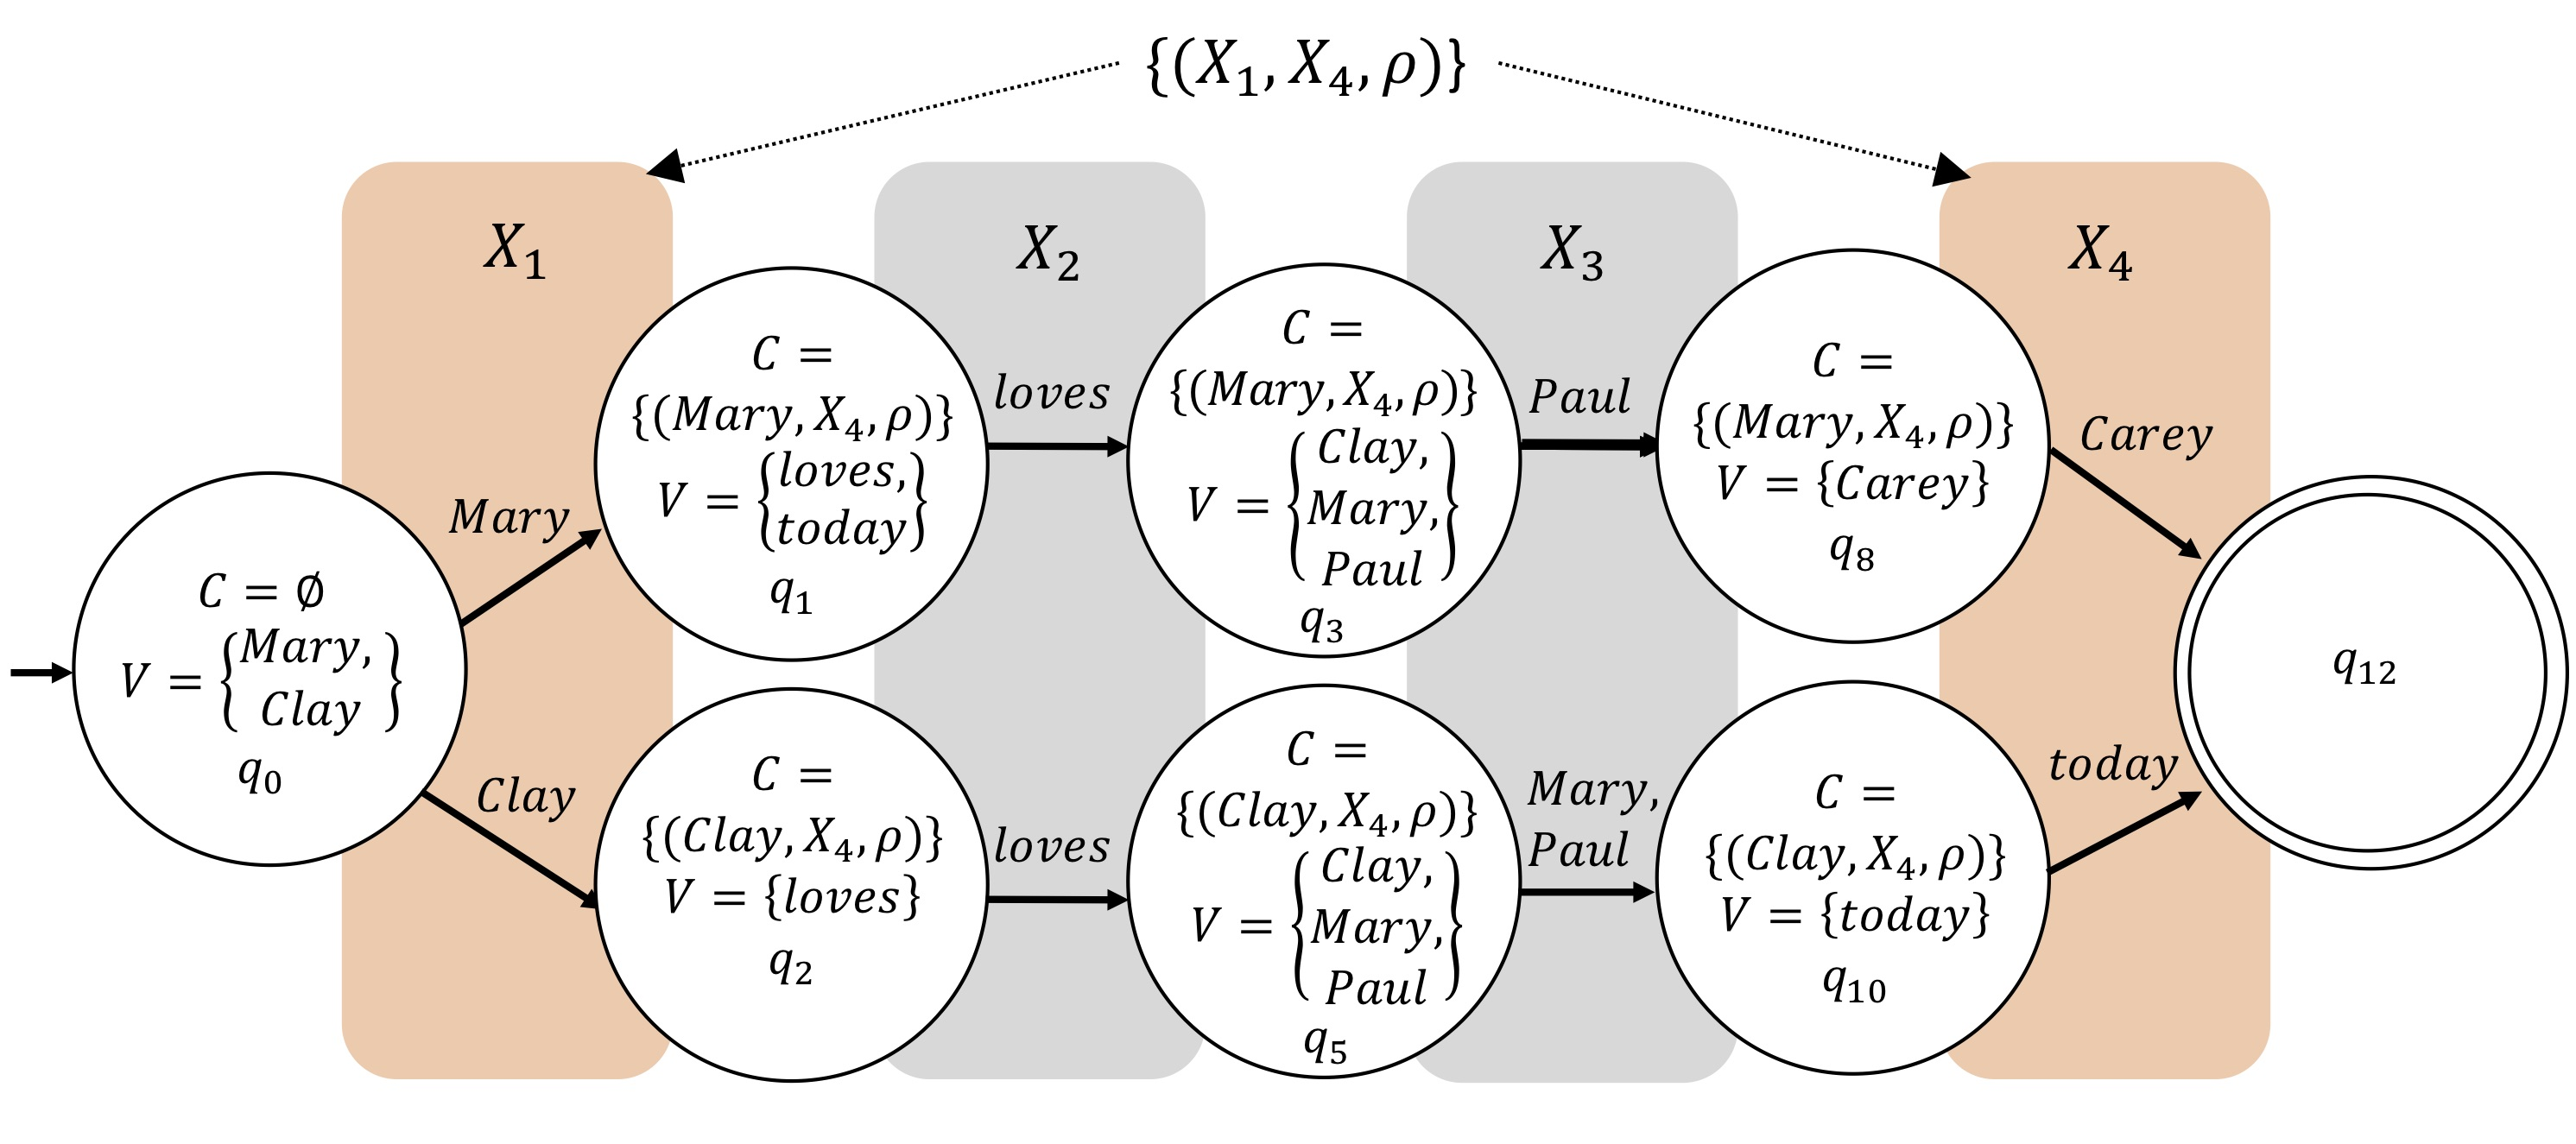
\includegraphics[width=\linewidth]{DFA}
	\caption{\label{fig:dfa} A DFA designed from a Markov model to accept sequences where the first and fourth words rhyme. The DFA is constructed breadth-first. By tracking constraints (the set $C$) and valid out-labels (the set $V$) at each state, the DFA avoids creating redundant states and ensures all paths satisfy relational constraints.}
\end{figure}

\section{Learning Relational Structure}

In the previous section we discussed a model that can generate sequences with relational structure (e.g., rhyme scheme, motifs, verse-chorus structure). These models presuppose a set of constraints representing the structure to be implemented. A system which generates novel, interesting structured sequences using manually-crafted structural constraints might be argued to exhibit creative behaviors; however, we can strengthen this argument by empowering the system with the ability to autonomously learn and generate its \emph{own} structural constraints.

To learn a model of relational structures we adapt the traditional Smith-Waterman (SW) algorithm for aligning sequences \cite{smite1981identification} in three ways. First, unlike its traditional use for aligning \emph{different} sequences, our modified \emph{multi-}SW (or mSW) \emph{self-}alignment algorithm is designed to align a sequence against itself for finding regions of \emph{self}-similarity. This adaptation requires computing only the upper diagonal of the alignment matrix, excluding the diagonal itself. Second, the mSW algorithm discovers not just the best local alignment, but all local alignments above a particular threshold. In allowing for this modification we require local alignment origins to be some minimal distance from one another to avoid confounding alignments. Third, the scoring function of two musical sequence events is custom-designed to consider factors relevant to the particular viewpoint structure being modeled (e.g., when learning rhythmic relational structure, factors might include metric position, note duration, rest vs. played, etc.). The factors are hand-picked (though they might just as easily be learned); however, the weights of each factor are learned via genetic algorithm using F-score accuracy on set of structurally labeled training instances as a fitness function.

For each of several viewpoints (e.g., harmony, melodic pitch, rhythm, and lyrics) we train a scoring function which can be used to detect relational structure in an arbitrary unlabeled lead sheet (see Figure~\ref{fig:structure}). This structure represents a set of learned constraints for imposing similar (viewpoint-specific) structure in novel compositions.

\begin{figure}
	\centering
	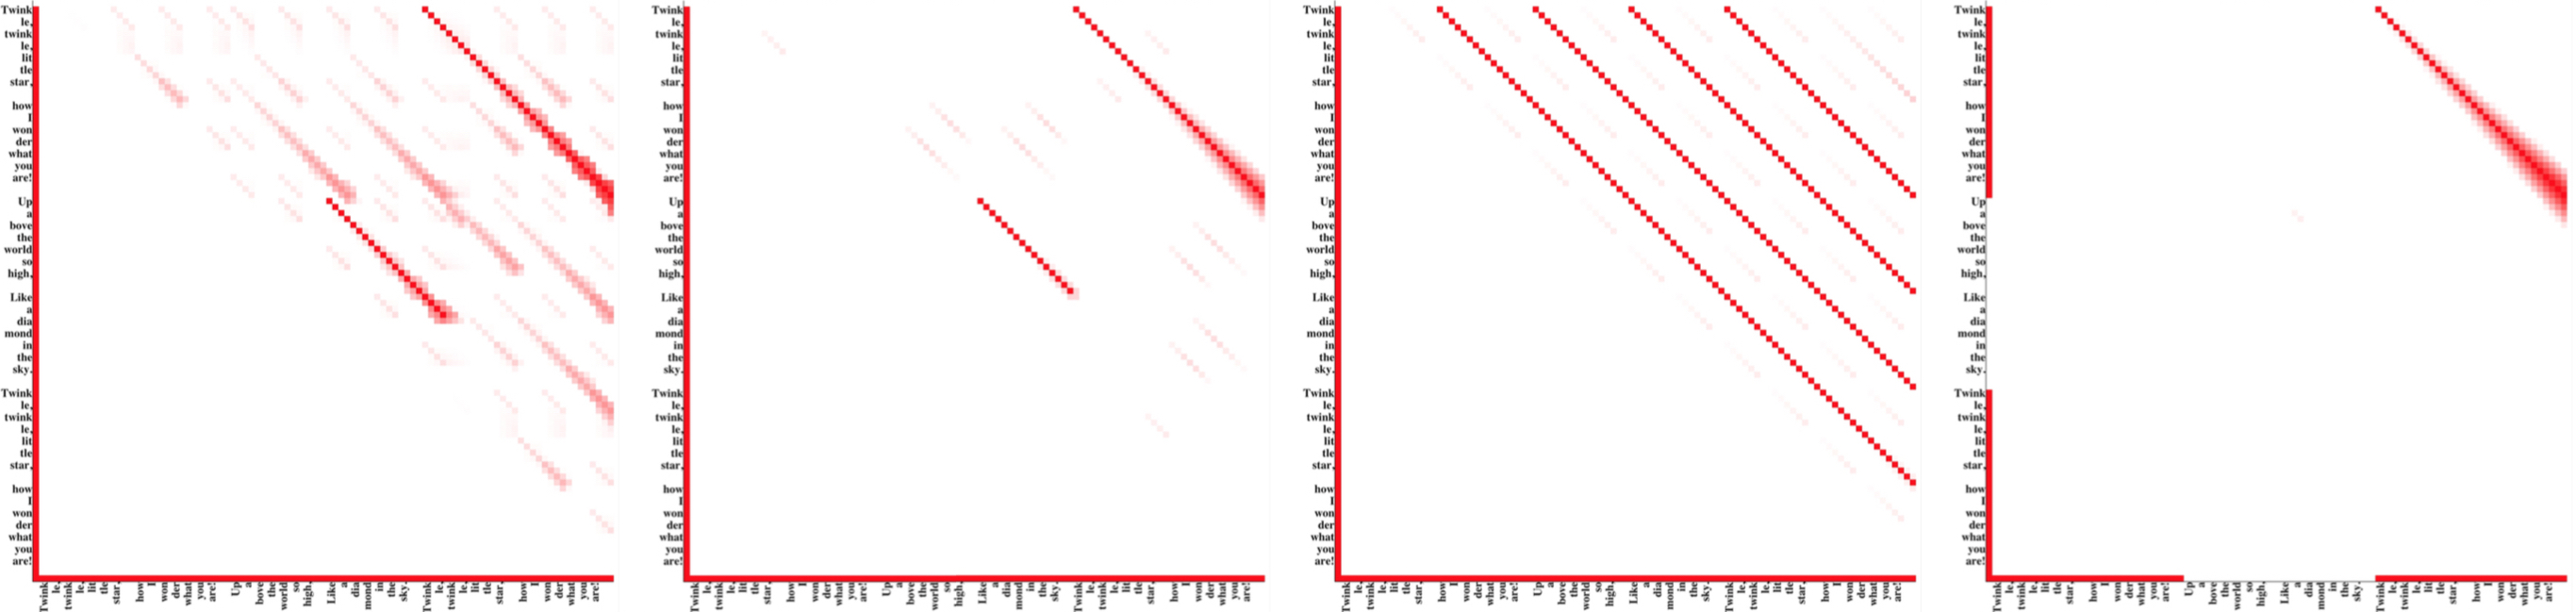
\includegraphics[width=\linewidth]{structure}
	\caption{\label{fig:structure} These alignment matrices were generated using the mSW alignment algorithm to find (from left to right) harmonic, pitch, rhythmic, and lyrical relational structure in \emph{Twinkle, Twinkle, Little Star}.}
\end{figure}

\section{Music with a Muse}

\begin{figure}[b!]
	\centering
	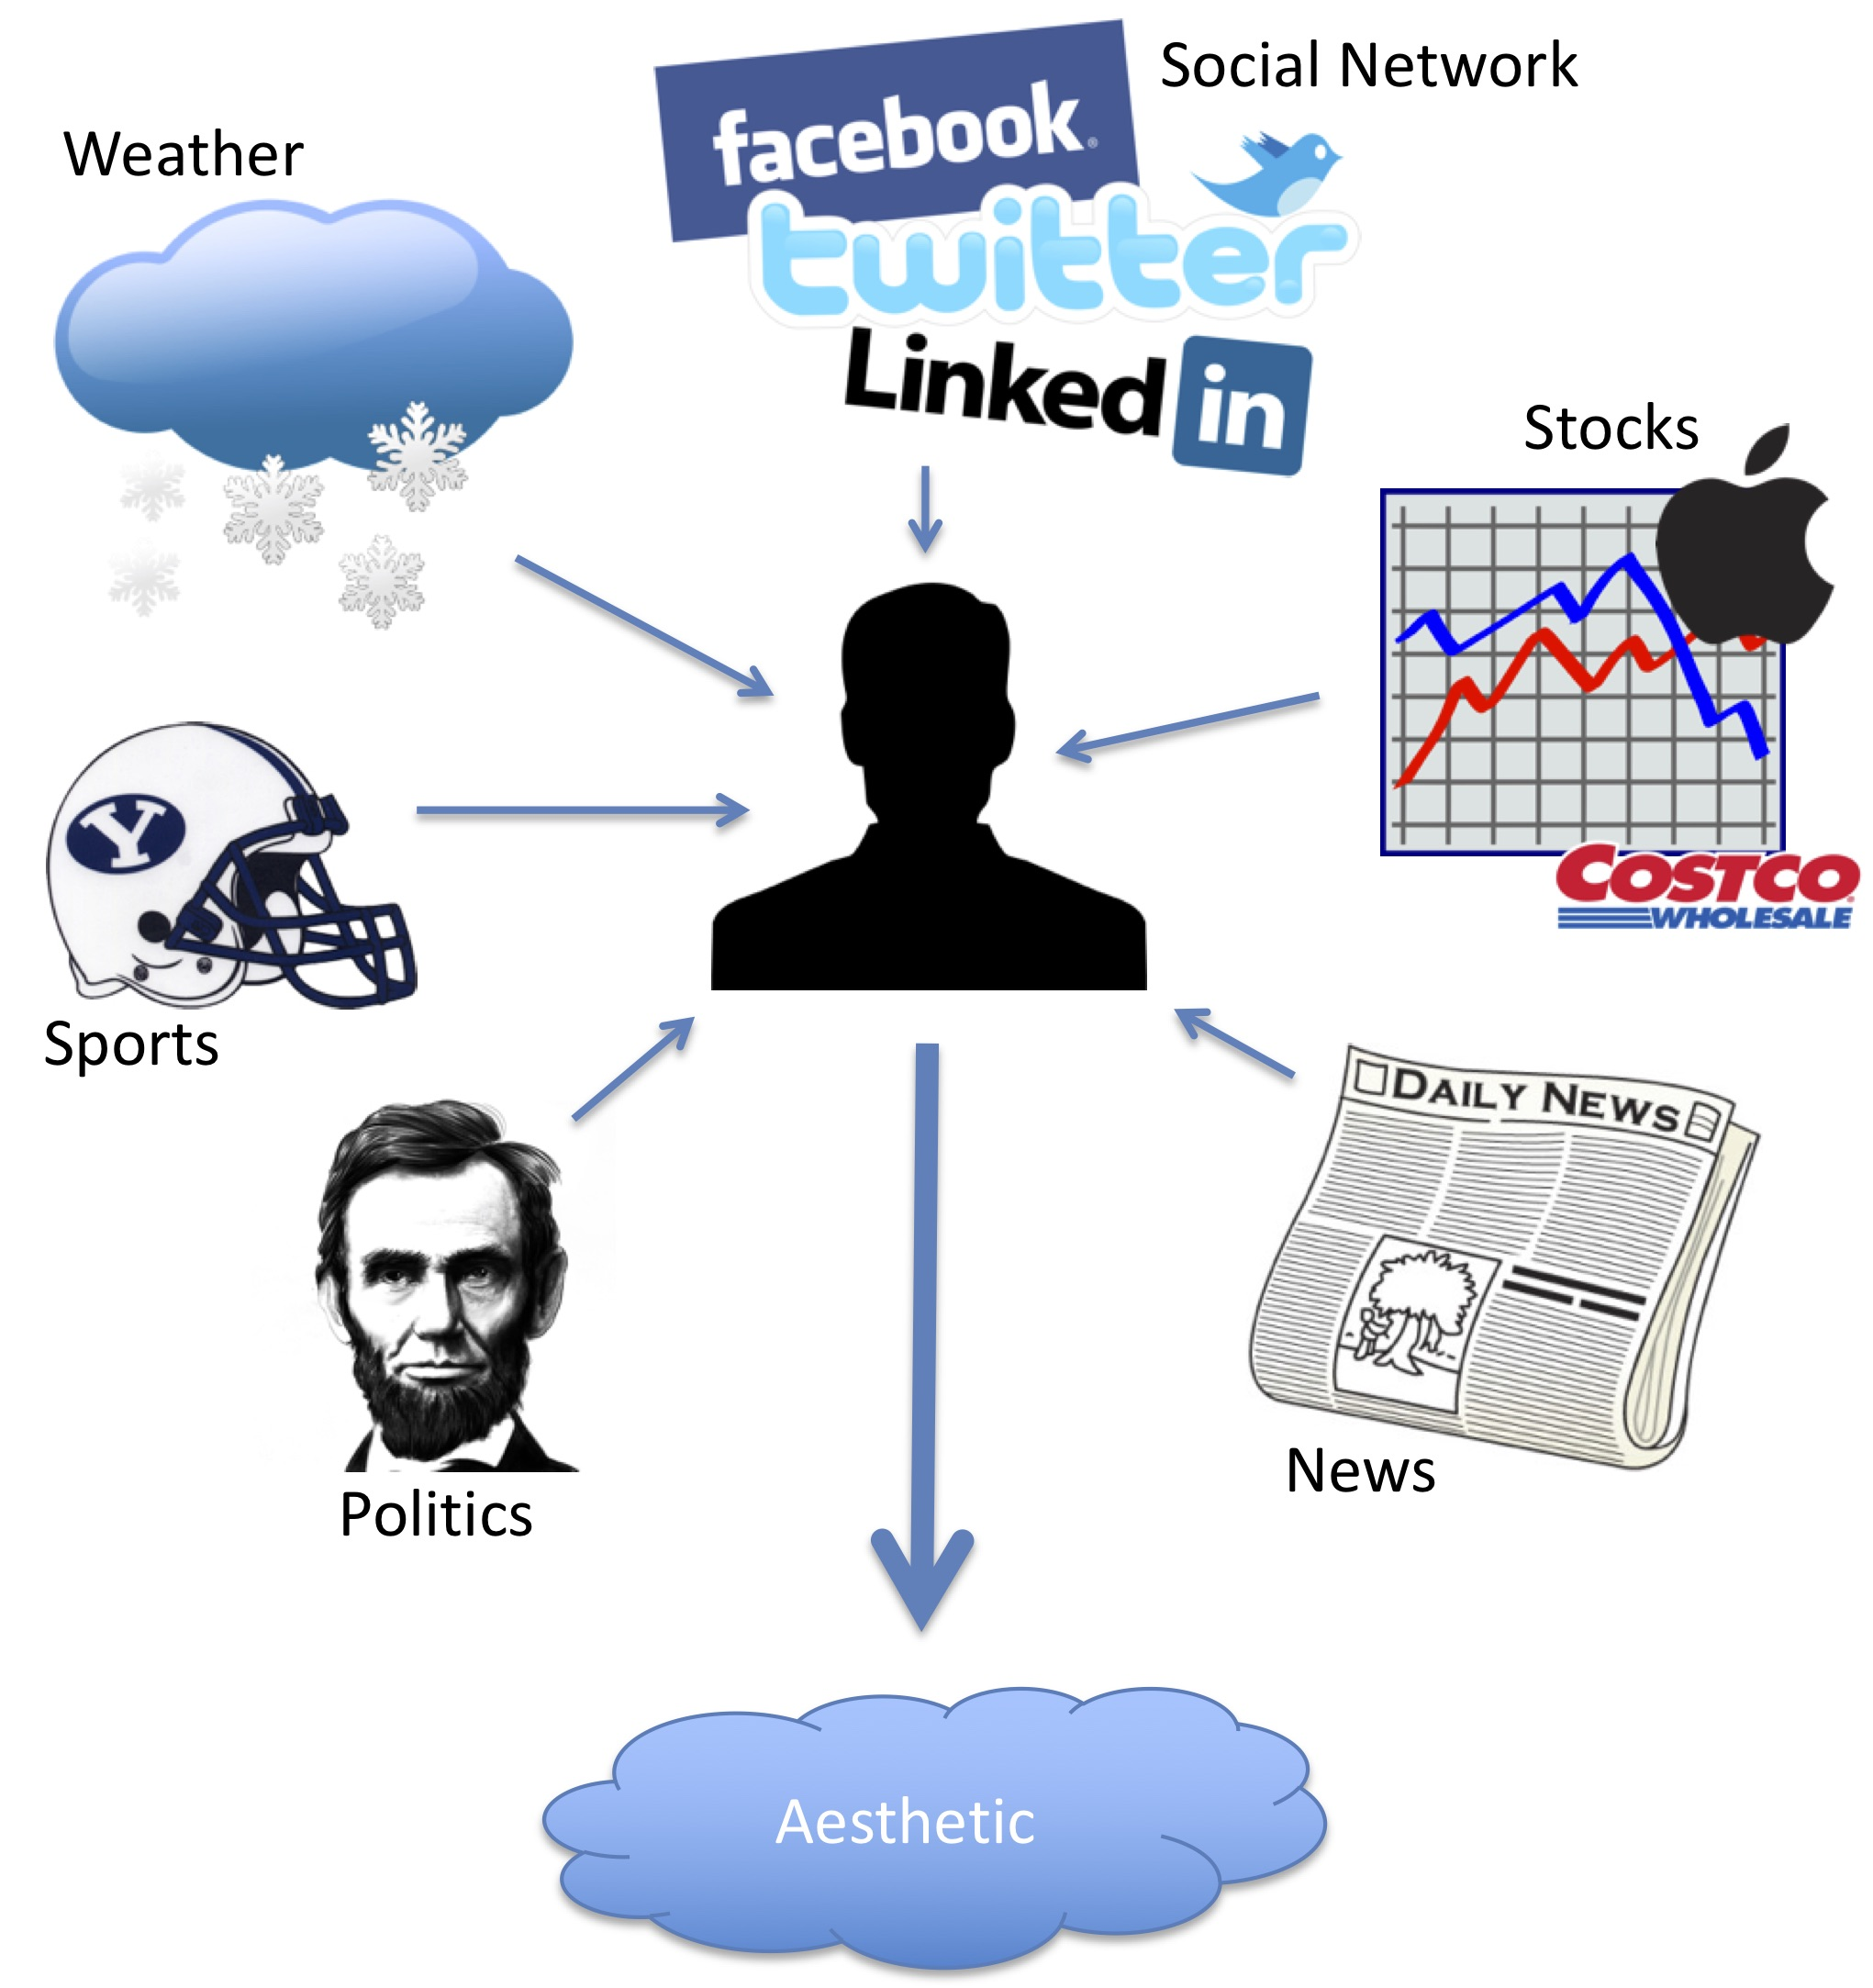
\includegraphics[width=.6\linewidth]{InspiringSources}
	\caption{\label{fig:inspiration} Similar to a human composer, the system derives inspiration from meaningful events related to aspects of its environment that it cares about or has preferences towards.}
\end{figure}

\begin{figure*}[t!]
	\centering
	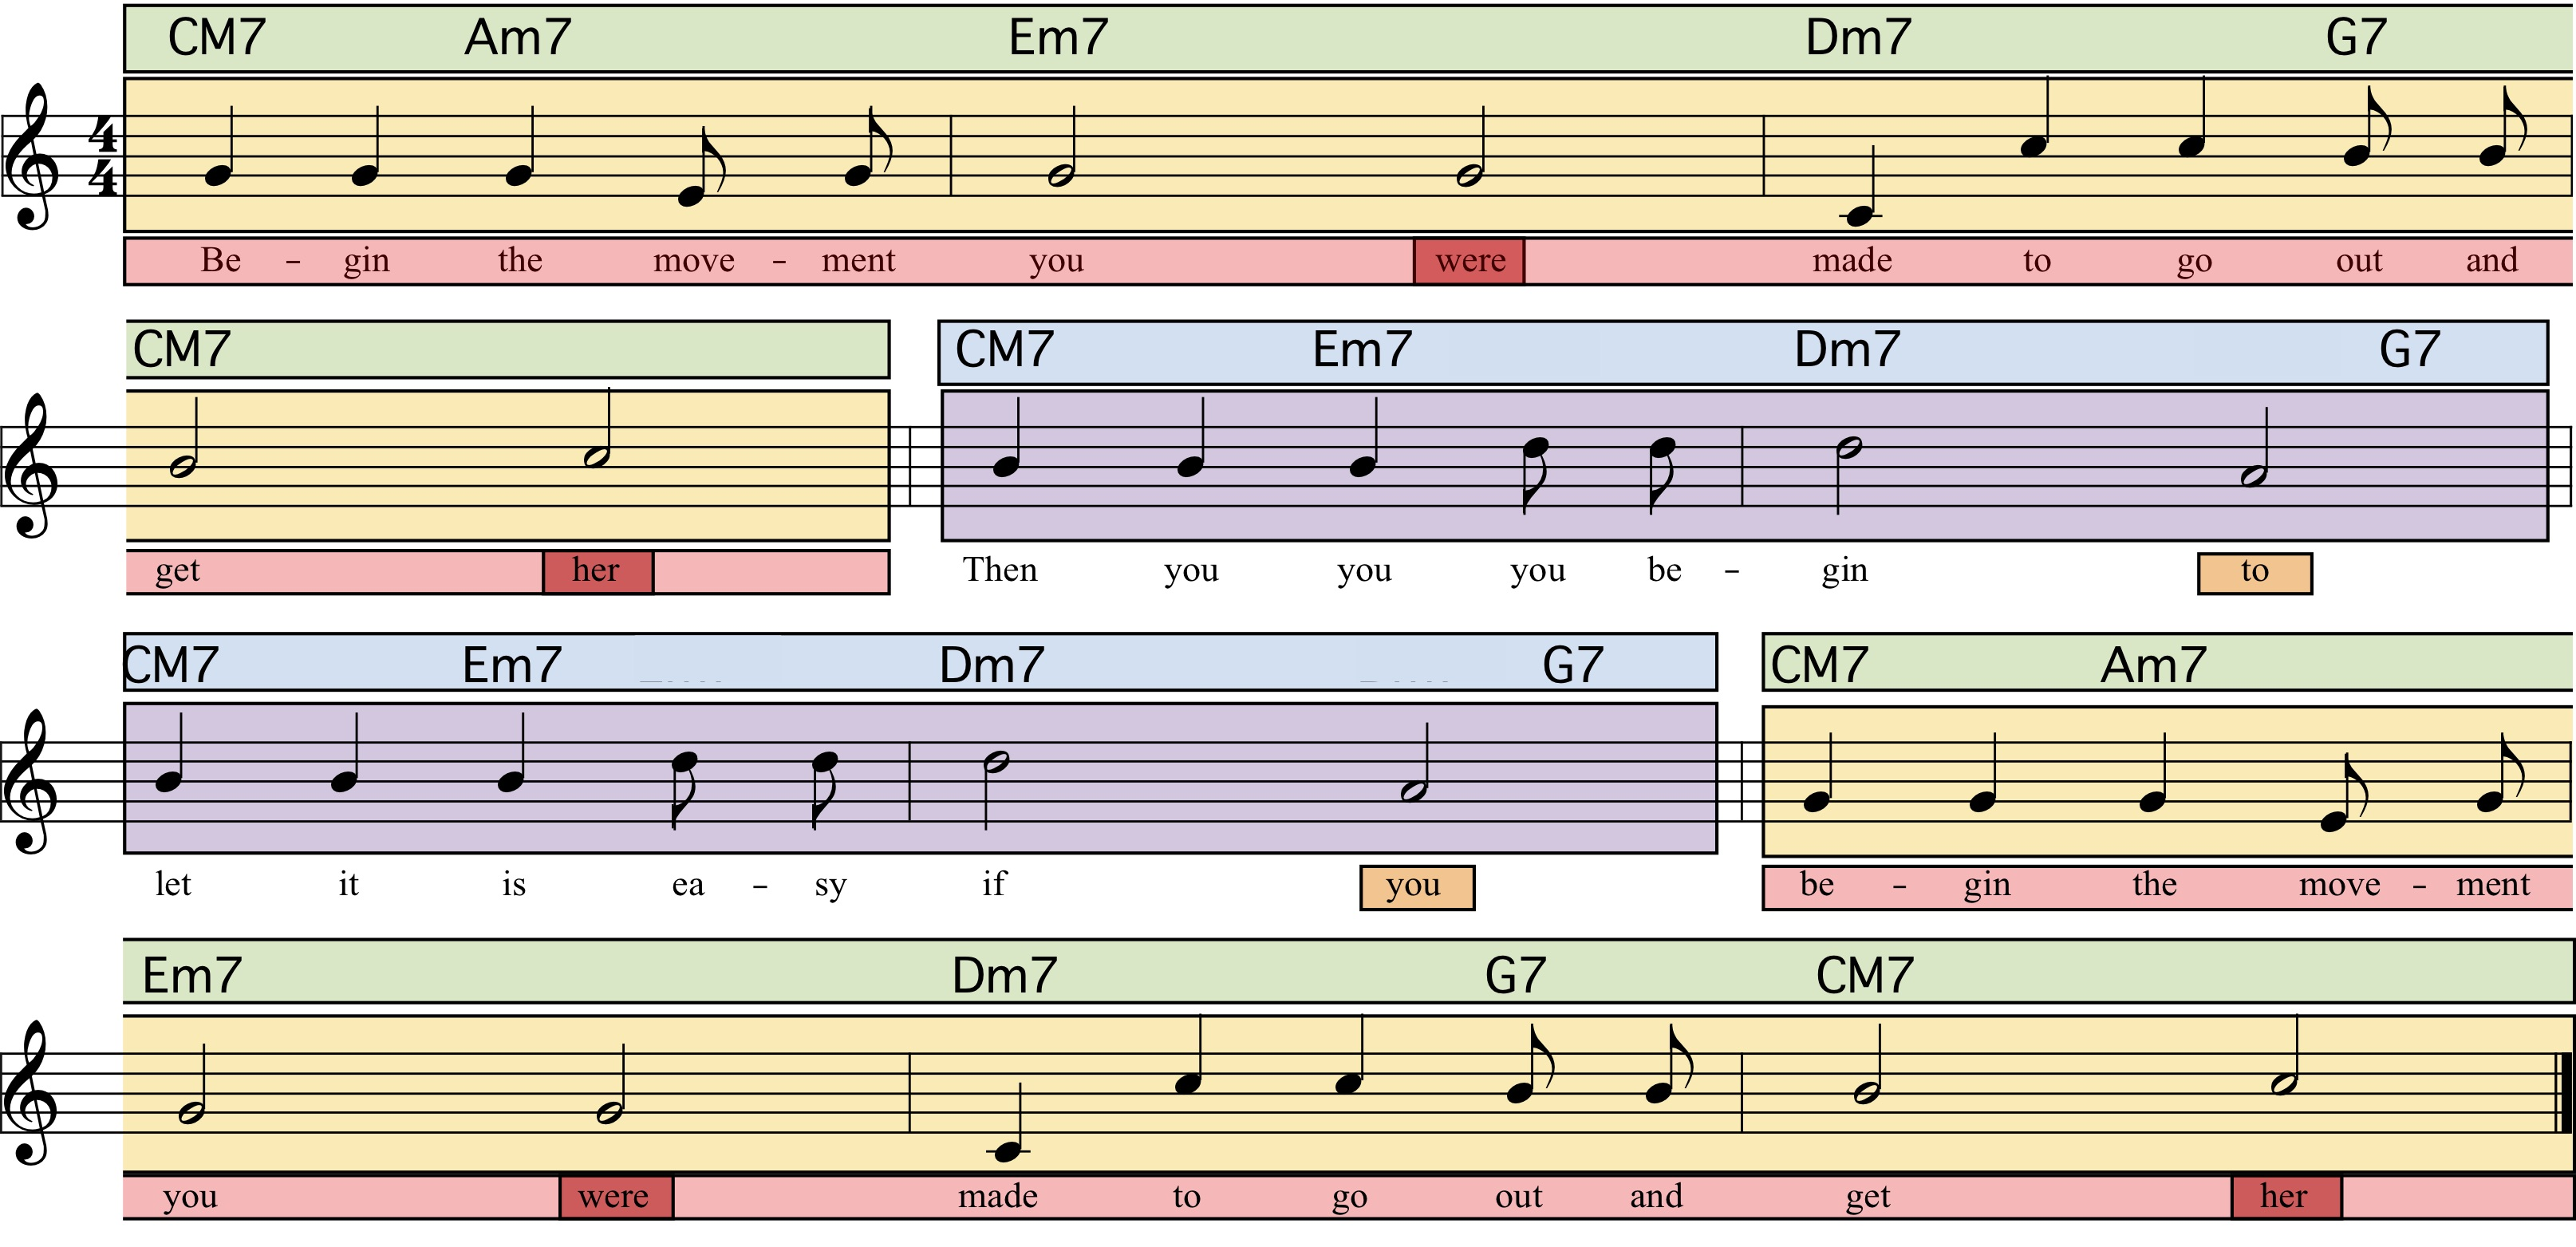
\includegraphics[width=.8\linewidth]{Song}
	\caption{\label{fig:song} The above composition (color-coded to highlight structural repetitions) is described by the system as follows: ``As one interested in Salt Lake weather, I stumbled on this tweet from Friday, May 04, 2018 at 12:21 AM by Black Barbie: `Keep me in yaw prayers I have a 3 your flight from Salt Lake City to Chicago and there is bad weather everywhere. The last time I flew in bad weather we were struck by lightning.' It got me thinking about weather and violence and ultimately led me to write this song. I intended that the piece should be about weather and violence, but in the end I felt that it was more about childish and love. In any case, I hope you find it meaningful.''}
\end{figure*}


The result of our contributions thus far have resulted in a system which is capable of generating relationally-structured sequences through autonomous learning of relational structure in existing music. This system, though thoroughly capable of creating well-structured music, lacks a key aspect of autonomous creative systems: intentionality. To effectively convince unbiased observers of its creative behavior, we add a third and final component which enables the computational composer not only to channel a particular idea or emotion, but also to effectively \emph{choose} this inspiration based on its preferences and its interaction with its environment.

The system is created with a set of \emph{preferences}: concepts, entities, and locations in which it is ``emotionally'' invested (see Figure~\ref{fig:inspiration}). For example, our system might hail from Salt Lake City, Utah, love the Utah Jazz, and be affected by the Salt Lake weather. For our purposes these preferences remain static through time, though one might speculate as to how they could evolve.

Given this set of preferences, the system is inspired by events that take place in relation to these preferences as the system learns about them through Twitter. For example, if the system sees a tweet that ``Rainy weather in Salt Lake City make me feel sad and gloomy!!'', then the system itself (with the help of the Empath algorithm \cite{fast2016empath}) is inspired with feelings of ``cold,'' ``sadness,'' and ``negative emotion''.

These feelings are converted into a novel musical composition using the process for generating structured sequences described above. In applying the process, Markov models are trained on songs in the corpus whose lyrics inspire the most similar feelings to those inspired by the observed tweet. The result is a well-structured, intention-driven, lyrical composition.


Because the system is able to analyze and assess the feelings evoked by particular tweets or lyrics, it is also able to self-reflect on the music that \emph{it} creates. Thus when the system generates a new song, it can explain \emph{why} it wrote the song and \emph{how successfully} it achieved its intentions (see Figure~\ref{fig:song}).  

\section{Conclusion}

A system capable of autonomously generating well-structured, intentioned music opens a myriad of possibilities including aids for learning and memory; tools for addressing depression and anxiety; and a creative collaborator and inspiration for musicians. Most integral to our purposes, however, is the progress that it represents and the questions it raises about the potential for computers to exhibit creative behavior. We are actively designing an empirical evaluation by which to demonstrate the meaningfulness, creativity, and impact of the system's creative process and output.

\bibliographystyle{iccc}
\bibliography{../all}


\end{document}
